\documentclass[conference]{IEEEtran}
\IEEEoverridecommandlockouts
\usepackage[utf8]{inputenc}
\usepackage[T1]{fontenc}
\usepackage{graphicx}
\usepackage{booktabs}
\usepackage{amsmath}
\usepackage{hyperref}

\def\IEEEbstctlcite#1{}

\begin{document}

% ---- Conference / copyright footer (EDIT to match your target venue's LaTeX kit) ----
\IEEEoverridecommandlockouts
\IEEEpubid{\makebox[\columnwidth]{978-1-XXXX-XXXX-X/25/\$31.00~\copyright{}2025 IEEE \hfill}
\hspace{\columnsep}\makebox[\columnwidth]{ }}

\title{Confidence-Gated Abstention for Reducing Hallucination in Retrieval-Augmented Generation}

\author{
\IEEEauthorblockN{
\begin{minipage}[t]{0.48\textwidth}
\centering
Harsh Srivastava\\
\textit{\footnotesize JSS Academy of Technical Education}\\
\footnotesize Noida, India\\
\footnotesize \href{https://orcid.org/0009-0002-4863-3539}{ORCID: 0009-0002-4863-3539}
\end{minipage}
\hfill
\begin{minipage}[t]{0.48\textwidth}
\centering
Shantanu Tiwari\\
\textit{\footnotesize JSS Academy of Technical Education}\\
\footnotesize Noida, India\\
\footnotesize \href{https://orcid.org/0009-0004-2842-0805}{ORCID: 0009-0004-2842-0805}
\end{minipage}
\\[1.5em]
\begin{minipage}[t]{0.48\textwidth}
\centering
Bhavya Mishra\\
\textit{\footnotesize JSS Academy of Technical Education}\\
\footnotesize Noida, India\\
\footnotesize \href{https://orcid.org/0009-0000-0280-4414}{ORCID: 0009-0000-0280-4414}
\end{minipage}
\hfill
\begin{minipage}[t]{0.48\textwidth}
\centering
Rishabh Jain\\
\textit{\footnotesize JSS Academy of Technical Education}\\
\footnotesize Noida, India\\
\footnotesize \href{https://orcid.org/0009-0005-7499-9480}{ORCID: 0009-0005-7499-9480}
\end{minipage}
}
}

\maketitle

\begin{abstract}
Retrieval-augmented generation (RAG) hallucinates less than a bare language model, but most deployed systems still answer even when retrieval returns nothing useful. A common remedy is to gate generation on retrieval confidence: average the similarity of the retrieved passages and refuse when that average falls below a threshold. We study where this stops working. Our corpus is 62 Wikipedia pages on the Indian Premier League split into 2{,}732 passages, and our query set is 160 questions hand-labelled for answerability: 18 unrelated to cricket, and 35 \emph{near-miss} questions that sound like plausible IPL questions the corpus cannot answer. The gate handles the first group perfectly and the second badly. Out-of-domain questions score 0.135--0.336 and are refused every time; near-miss questions score 0.462--0.715 and sit inside the answerable range (0.517--0.824), so 74 of our 90 answerable questions score no higher than the best near-miss. No threshold separates them. At $\tau^\ast = 0.62$, selected by maximising abstention F1, the mechanism reaches F1 = 0.77 and MCC = 0.65 against a chance-matched baseline of 0.35 and 0.00, but recall on unanswerable questions is only 0.72. Faithfulness rises from 2.19 to 4.44 out of 5 against a no-context baseline and the hallucination rate falls from 99/160 to 7/84. Two methodological findings also emerged: the judge scores the identical refusal \texttt{"I don't know."} as faithfulness 1, 3 and 5 at temperature zero, forcing refusals out of any meaningful hallucination rate; and against 15 hand-scored items it agrees substantially with a human rater ($r = 0.83$ and $0.85$).
\end{abstract}

\begin{IEEEkeywords}
retrieval-augmented generation, hallucination, abstention, selective prediction, LLM-as-judge
\end{IEEEkeywords}

\section{Introduction}

Ask a language model something it does not know and it will usually answer anyway, fluently and confidently and often wrongly. This behaviour, generally filed under hallucination \cite{ji2023survey}, is the main reason such systems are awkward to deploy where a confident falsehood costs more than an admission of ignorance. Retrieval-augmented generation \cite{lewis2020rag} was meant to relieve the pressure: put relevant text in front of the model and it has less room to invent. In practice most RAG systems still answer when retrieval has failed, falling back on pretrained knowledge or inventing outright, and nothing in the output distinguishes that case from a grounded answer.

The obvious response, and the one we study, is to let the system decline. Average the similarity scores of the top-$k$ passages into one confidence number, compare it against a threshold, and refuse when it falls short. The mechanism is about as simple as possible, which is the point: one comparison, no training, and it attaches to any retriever that returns scores.

What we set out to find was not whether this helps, because it plainly does, but where its limits are. That depends almost entirely on how the evaluation set is built, and this is where work on the topic tends to go wrong: if the unanswerable questions are all obviously off-topic, the retriever separates them trivially, every abstention metric saturates, and the mechanism looks better than it is. Our contributions follow from avoiding that trap. We build a 160-question set with a deliberate difficulty gradient in the unanswerable class --- 18 off-topic questions and 35 \emph{near-miss} questions concerning the corpus's own subject but asking for what it does not hold --- and show that confidence separates the first group perfectly and the second not at all. We score the abstention decision as classification against ground truth and against a chance-matched random baseline, select the threshold by an explicit rule, compare three confidence definitions, and validate the judge against human ratings, documenting a failure mode that changes how the headline reliability metric must be computed. This is not a new mechanism: the value we claim lies in the measurement rather than the machinery.

\section{Related Work}

Lewis et al. \cite{lewis2020rag} introduced RAG with a dense retriever and generator trained jointly. What we build is less ambitious: a frozen sentence-embedding retriever feeding an off-the-shelf instruction-tuned model through an API, with no training in the loop --- less a step backwards than a description of how most RAG systems are actually assembled today.

The idea that a model should be allowed to say it does not know goes back to selective classification, and reached question answering when SQuAD 2.0 \cite{rajpurkar2018know} added unanswerable questions to a benchmark that had previously guaranteed an answer existed. That lesson carries over directly: an evaluation set containing only answerable questions says nothing about a system's willingness to refuse. Ours is close to the most primitive version, using the retriever's own similarity with no learned answerability classifier. More elaborate approaches exist --- Self-RAG \cite{asai2024selfrag} trains a model to emit reflection tokens deciding when to retrieve and whether the retrieved text supports generation --- but our interest is in what the cheapest signal buys, since that sets the floor such methods must beat.

Hallucination is broad enough to need a survey \cite{ji2023survey}; our faithfulness measure touches one corner, namely whether an answer is supported by the passages it was handed. An answer can be true about the world and still unsupported by the retrieved text, and that distinction matters throughout. Calibration is the neighbouring concern: Guo et al. \cite{guo2017calibration} showed modern networks are systematically overconfident and Kadavath et al. \cite{kadavath2022know} that language models carry some signal about their own correctness. Our score is calibrated in neither sense. Infrastructure is unremarkable: Sentence-BERT \cite{reimers2019sentencebert} embeddings, a FAISS \cite{johnson2019faiss} index. Grading one model's output with another is now standard \cite{zheng2023judging}, and frameworks such as RAGAs \cite{es2024ragas} build RAG-specific metrics on it; we use a judge for the same reason but decline to assume it works (Section \ref{sec:judge-validation}).

\section{Method}

\subsection{System Overview and Confidence Score}

A query is embedded and used to retrieve the top-$k$ passages; their similarity scores are collapsed into one confidence number; that number is compared against a threshold; the system either generates from the retrieved context or emits a fixed refusal; and the output is scored.

The corpus is prepared once, offline: sections split into overlapping character chunks, embedded, and stored in a FAISS \texttt{IndexFlatIP} index over L2-normalised vectors, so the inner product is cosine similarity. At query time the same model encodes the question and the index returns its $k = 3$ nearest chunks in descending order.

For a query $q$ retrieving passages with scores $\{s_1, \ldots, s_k\}$, confidence is the mean:
\begin{equation}
c(q) = \frac{1}{k}\sum_{i=1}^{k} s_i .
\end{equation}
If $c(q) < \tau$ the system abstains, returning \emph{``I don't know based on the provided context.''} We swept $\tau$ over sixteen values from 0.10 to 0.80, chosen to bracket both edges of the useful range.

\subsection{Alternative Confidence Definitions}
\label{sec:variants}

The mean is arbitrary, so we tested two alternatives: a rank-weighted score $c_{\text{w}}(q) = 0.5 s_1 + 0.3 s_2 + 0.2 s_3$, on the intuition that the top hit should count for more, and the maximum $c_{\max}(q) = \max_i s_i$, on the intuition that one relevant passage suffices. Since neither changes what was retrieved or generated, all three evaluate from a single cached run.

\subsection{Threshold Selection}
\label{sec:threshold-selection}

Picking $\tau$ by eye off a plot is not reproducible, so we define it as an optimisation. Every query carries a label $a(q) \in \{\text{true}, \text{false}, \text{uncertain}\}$ recording whether the corpus can answer it. Treating $a(q) = \text{false}$ as the positive class and restricting to definite labels,
\begin{equation}
\tau^\ast = \arg\max_\tau \; F_1^{\text{abstain}}(\tau).
\end{equation}
Ties are broken by a coverage-weighted quality score, the harmonic mean of coverage and effective relevance rescaled to $[0,1]$, and any residual tie by preferring the lowest $\tau$. The rule lives in a standalone script, so the choice can be re-run and checked.

Neither retrieval nor generation depends on $\tau$, so each query is run once and the sweep derived afterwards by masking on cached confidences. Besides being roughly $k$ times cheaper, this makes the sweep exact: re-judging at every threshold would let judge nondeterminism move the faithfulness column independently of the variable under study.

\subsection{Models}

Generation uses Groq-hosted \texttt{openai/gpt-oss-20b} and evaluation \texttt{openai/gpt-oss-120b} as the judge, held fixed across every experiment so all scores are comparable; using a larger model to grade a smaller one also avoids a generator marking its own work. Both run at temperature 0 with \texttt{max\_tokens} 1024, which matters because the \texttt{gpt-oss} family spend completion tokens on a separate \texttt{reasoning} field and a tighter limit returns empty content.

\section{Experimental Setup}

\subsection{Corpus and Query Set}

We scraped 62 Wikipedia pages covering the IPL --- the league and its governing body, all ten current franchises, five defunct ones, twenty players, six seasons, four records pages, eight venues, and surrounding cricket context --- yielding 823 sections split into 2{,}732 passages of roughly 500 characters with 100 of overlap. The IPL was chosen because it is factually dense and bounded sharply enough that we could decide by hand which questions the corpus can answer; without that, the ground-truth labels and every abstention metric here would be impossible. One scraping detail matters: sections are collected recursively, since a Wikipedia heading such as \emph{History} usually holds no prose itself and a top-level walk discards most of every page.

We wrote 160 questions by hand, each tagged with a category and answerability label (Table \ref{tab:queryset}). Ninety are ordinary in-domain questions --- factual lookups, reasoning, comparisons, numeric --- labelled \emph{true}. Eighteen have nothing to do with cricket (\emph{``What is the capital of Mongolia?''}) and are labelled \emph{false}; in earlier versions of this work these were the only unanswerable questions, which turned out to be the flaw.

Thirty-five are \emph{near-miss}: they sound like reasonable IPL questions but ask for what Wikipedia does not carry. They fall into families --- the future (\emph{``Which players will Chennai Super Kings retain for the 2027 auction?''}), hyper-specific statistics (\emph{``What was Bumrah's economy rate in powerplay overs during the 2022 IPL?''}), behind-the-scenes matters, granular match details, obscure conditional records, and confidential commercial information. These are labelled \emph{false} and are the heart of the evaluation. A further seventeen are \emph{in-domain hard}: IPL questions asking for exact figures Wikipedia sometimes carries and sometimes does not. We could not certify these either way, so they are labelled \emph{uncertain} and excluded from every abstention metric, though still generated and scored.

Every label was checked against the corpus: for answerable questions we confirmed the supporting text exists, and for near-miss questions we read the passages the retriever returns and confirmed the answer is absent. That check caught one mistake: we had written \emph{``What do cricket experts think about the impact player rule?''} as a near-miss, assuming Wikipedia does not editorialise. It does, so the question was answerable and we replaced it.

\begin{table}[htbp]
\centering
\caption{Query set composition (N = 160)}
\label{tab:queryset}
\begin{tabular}{@{}lccl@{}}
\toprule
Category & $n$ & Answerable & Purpose \\
\midrule
Factual & 40 & true & retrieval/generation \\
Reasoning & 20 & true & retrieval/generation \\
Comparative & 15 & true & retrieval/generation \\
Numeric & 15 & true & retrieval/generation \\
In-domain hard & 17 & uncertain & stress test \\
Near-miss & 35 & false & abstention (hard) \\
Out-of-domain & 18 & false & abstention (easy) \\
\midrule
\multicolumn{2}{@{}l}{Labelled for abstention scoring} & 143 & \\
\bottomrule
\end{tabular}
\end{table}

\subsection{Baseline and Metrics}
\label{sec:metrics}

The baseline is the same generation model handed the question with no context and no option to abstain, which isolates grounding as the variable. It is judged against the same retrieved context the RAG system received, which is what makes the two faithfulness columns comparable: faithfulness asks whether an answer is supported by the passages, not whether it is true in the world, and this is how an ungrounded but factually correct answer earns a low score.

Relevance and faithfulness are scored 1--5 by the judge, with an abstention assigned relevance 1 and faithfulness 5 without consulting it. \emph{Effective} relevance and faithfulness average over answered queries only, and we report these throughout, since the overall faithfulness number is inflated by the rule that hands every abstention a 5. Hit@$k$, Precision@$k$ and MRR@$k$ use keyword matching over the 90 answerable queries. Abstention precision, recall, F1, specificity and accuracy take ``should abstain'' as the positive class over the 143 definitely-labelled queries, alongside the Matthews correlation coefficient, which uses all four cells of the confusion matrix and so penalises both error types proportionally under imbalance:
\begin{equation}
\text{MCC} = \frac{\text{TP}\!\cdot\!\text{TN} - \text{FP}\!\cdot\!\text{FN}}
{\sqrt{(\text{TP}+\text{FP})(\text{TP}+\text{FN})(\text{TN}+\text{FP})(\text{TN}+\text{FN})}} .
\end{equation}
The hallucination rate is the share of substantive answers scored below 3 on faithfulness, with refusals excluded from numerator and denominator for reasons given in Section \ref{sec:refusals}.

\section{Results}

\subsection{RAG With Abstention Against the Baseline}

Table \ref{tab:baseline} and Fig. \ref{fig:final} set RAG at $\tau^\ast = 0.62$ against the no-context baseline. Faithfulness more than doubles, 2.19 to 4.44; restricted to answered queries, so the abstention rule contributes nothing, it is still 4.18. The hallucination rate puts it more bluntly: 7 unfaithful answers out of 84 substantive ones, against 99 of 160 for the baseline. The baseline wins on raw relevance, 4.23 to 3.08, which is not a defect in the RAG system: it answers all 160 questions, including the 53 it has no grounding for, fluently and from pretrained knowledge --- exactly the behaviour faithfulness exists to catch. Among the 109 questions RAG answered, its relevance is 4.06.

\begin{table}[htbp]
\centering
\caption{RAG with abstention vs.\ no-context baseline (N = 160, $\tau^\ast = 0.62$)}
\label{tab:baseline}
\begin{tabular}{@{}lcc@{}}
\toprule
Metric & RAG & Baseline \\
\midrule
Relevance (all 160) & 3.08 & \textbf{4.23} \\
Relevance (answered only, $n = 109$) & 4.06 & -- \\
Faithfulness (all 160) & \textbf{4.44} & 2.19 \\
Faithfulness (answered only) & 4.18 & -- \\
Hallucinations (faithfulness $< 3$) & \textbf{7/84} & 99/160 \\
Hallucination rate & \textbf{0.08} & 0.62 \\
Abstain rate & 0.32 & 0.00 \\
Generator-side refusals & 25/109 & -- \\
\bottomrule
\end{tabular}
\end{table}

\begin{figure}[htbp]
\centering
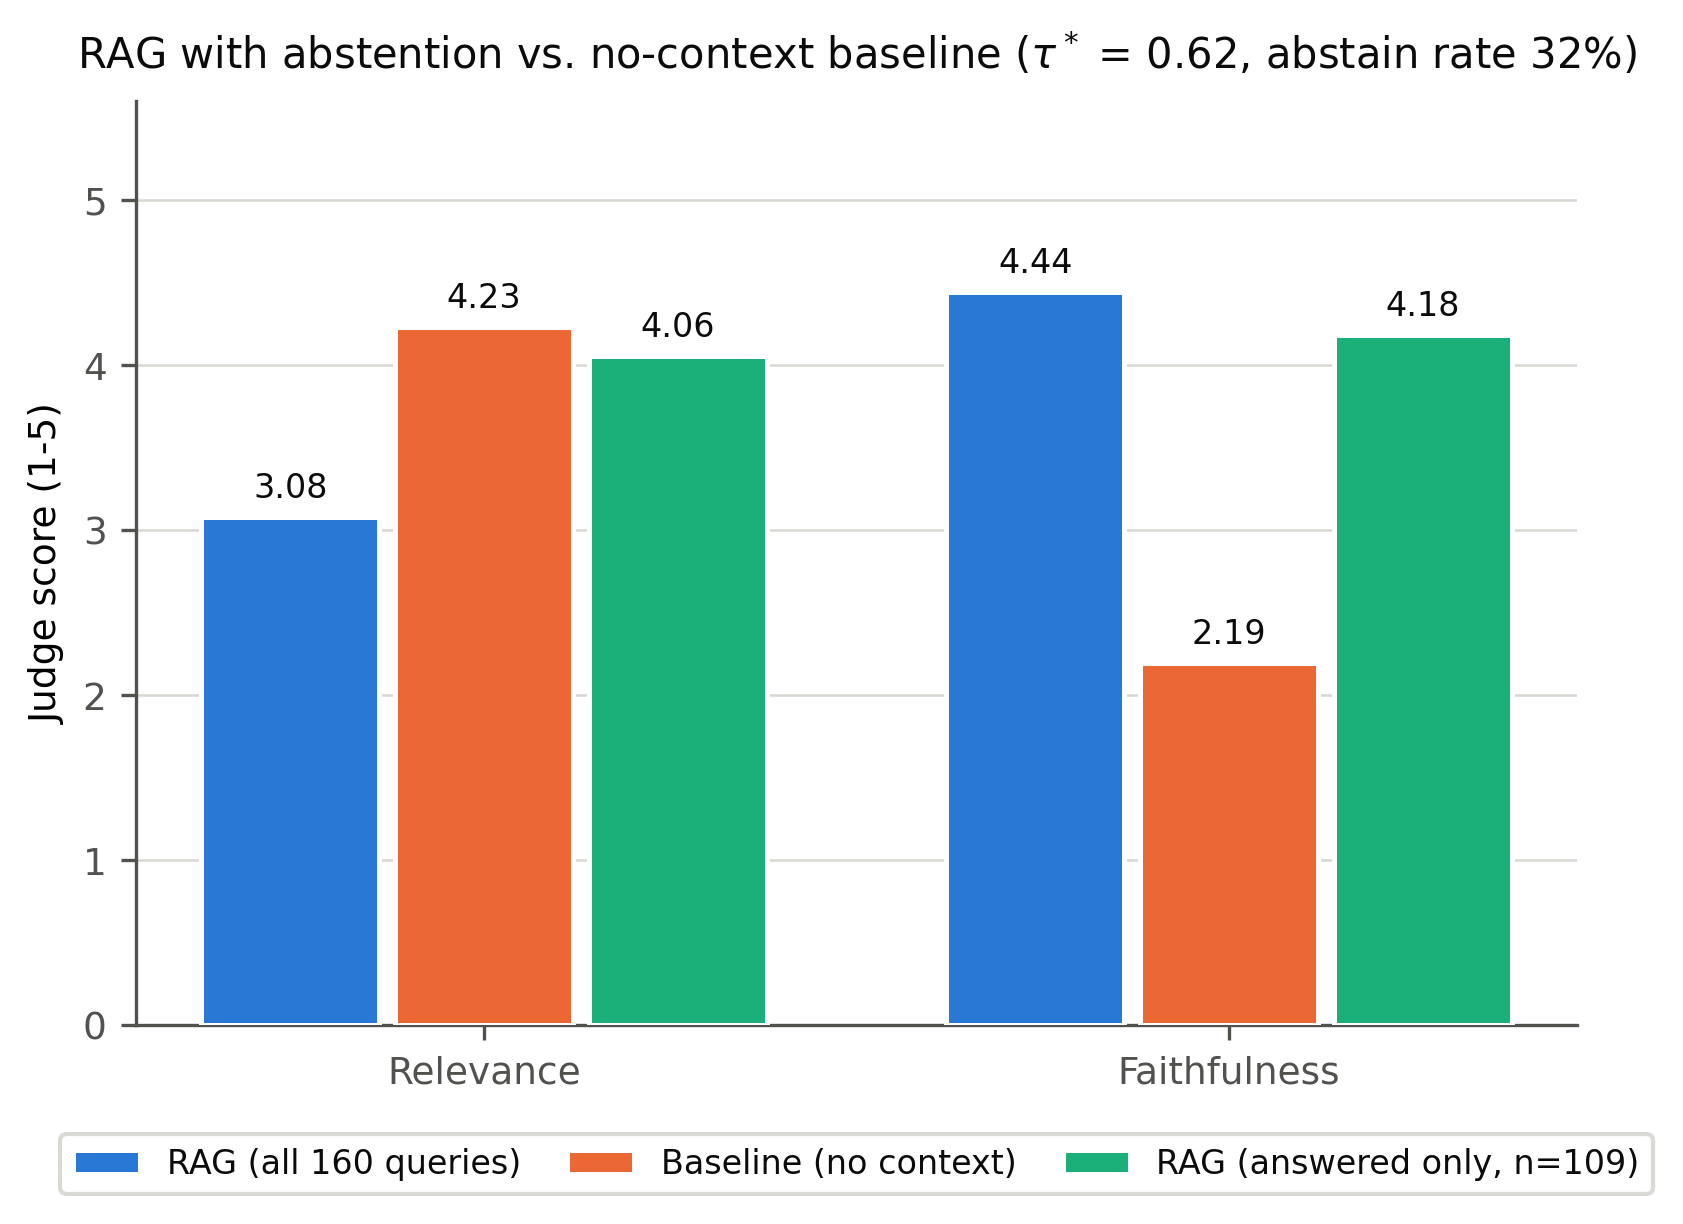
\includegraphics[width=\linewidth]{figures/final_plot.png}
\caption{RAG with abstention against the no-context baseline. Answered-only bars exclude the 51 abstentions, removing the contribution of the rule that assigns every abstention a faithfulness of 5.}
\label{fig:final}
\end{figure}

\subsection{Retrieval Quality}

Over the 90 answerable queries, Hit@3 is 0.93, Precision@3 is 0.73 and MRR@3 is 0.85: retrieval finds a relevant passage for most answerable questions and usually ranks it first. None vary with $\tau$, which is structural --- the threshold governs whether context is used, not what is retrieved. The residual 0.27 in Precision@3 matters more: roughly one passage in three reaching the generator is irrelevant, and that is the raw material for the failures in Section \ref{sec:failures}.

\subsection{What the Confidence Score Actually Separates}
\label{sec:separation}

This is the central result, and Fig. \ref{fig:confidence} carries it: plotting confidence by ground-truth class gives two completely different pictures depending on which unanswerable class you look at.

Out-of-domain questions score 0.135--0.336 and answerable questions 0.517--0.824. Nothing falls in the 0.18-wide band between, so any threshold inside it classifies all 108 of those queries correctly. For this class the mechanism is exact.

Near-miss questions score 0.462--0.715, inside the answerable range. Seventy-four of the 90 answerable questions score no higher than the best near-miss. There is no gap to place a threshold in, so whatever $\tau$ is chosen, refusing more near-miss questions means refusing answerable ones at close to the same rate.

The reason is not mysterious. Retrieval similarity measures topical proximity and a near-miss question is topically proximate by construction: asking for Bumrah's powerplay economy rate retrieves passages about his economy rate in other contexts, an excellent topical match containing nothing that answers the question. The score cannot see the difference because the difference is not topical --- it is whether a specific claim is present, and similarity does not encode that.

\begin{figure*}[t]
\centering
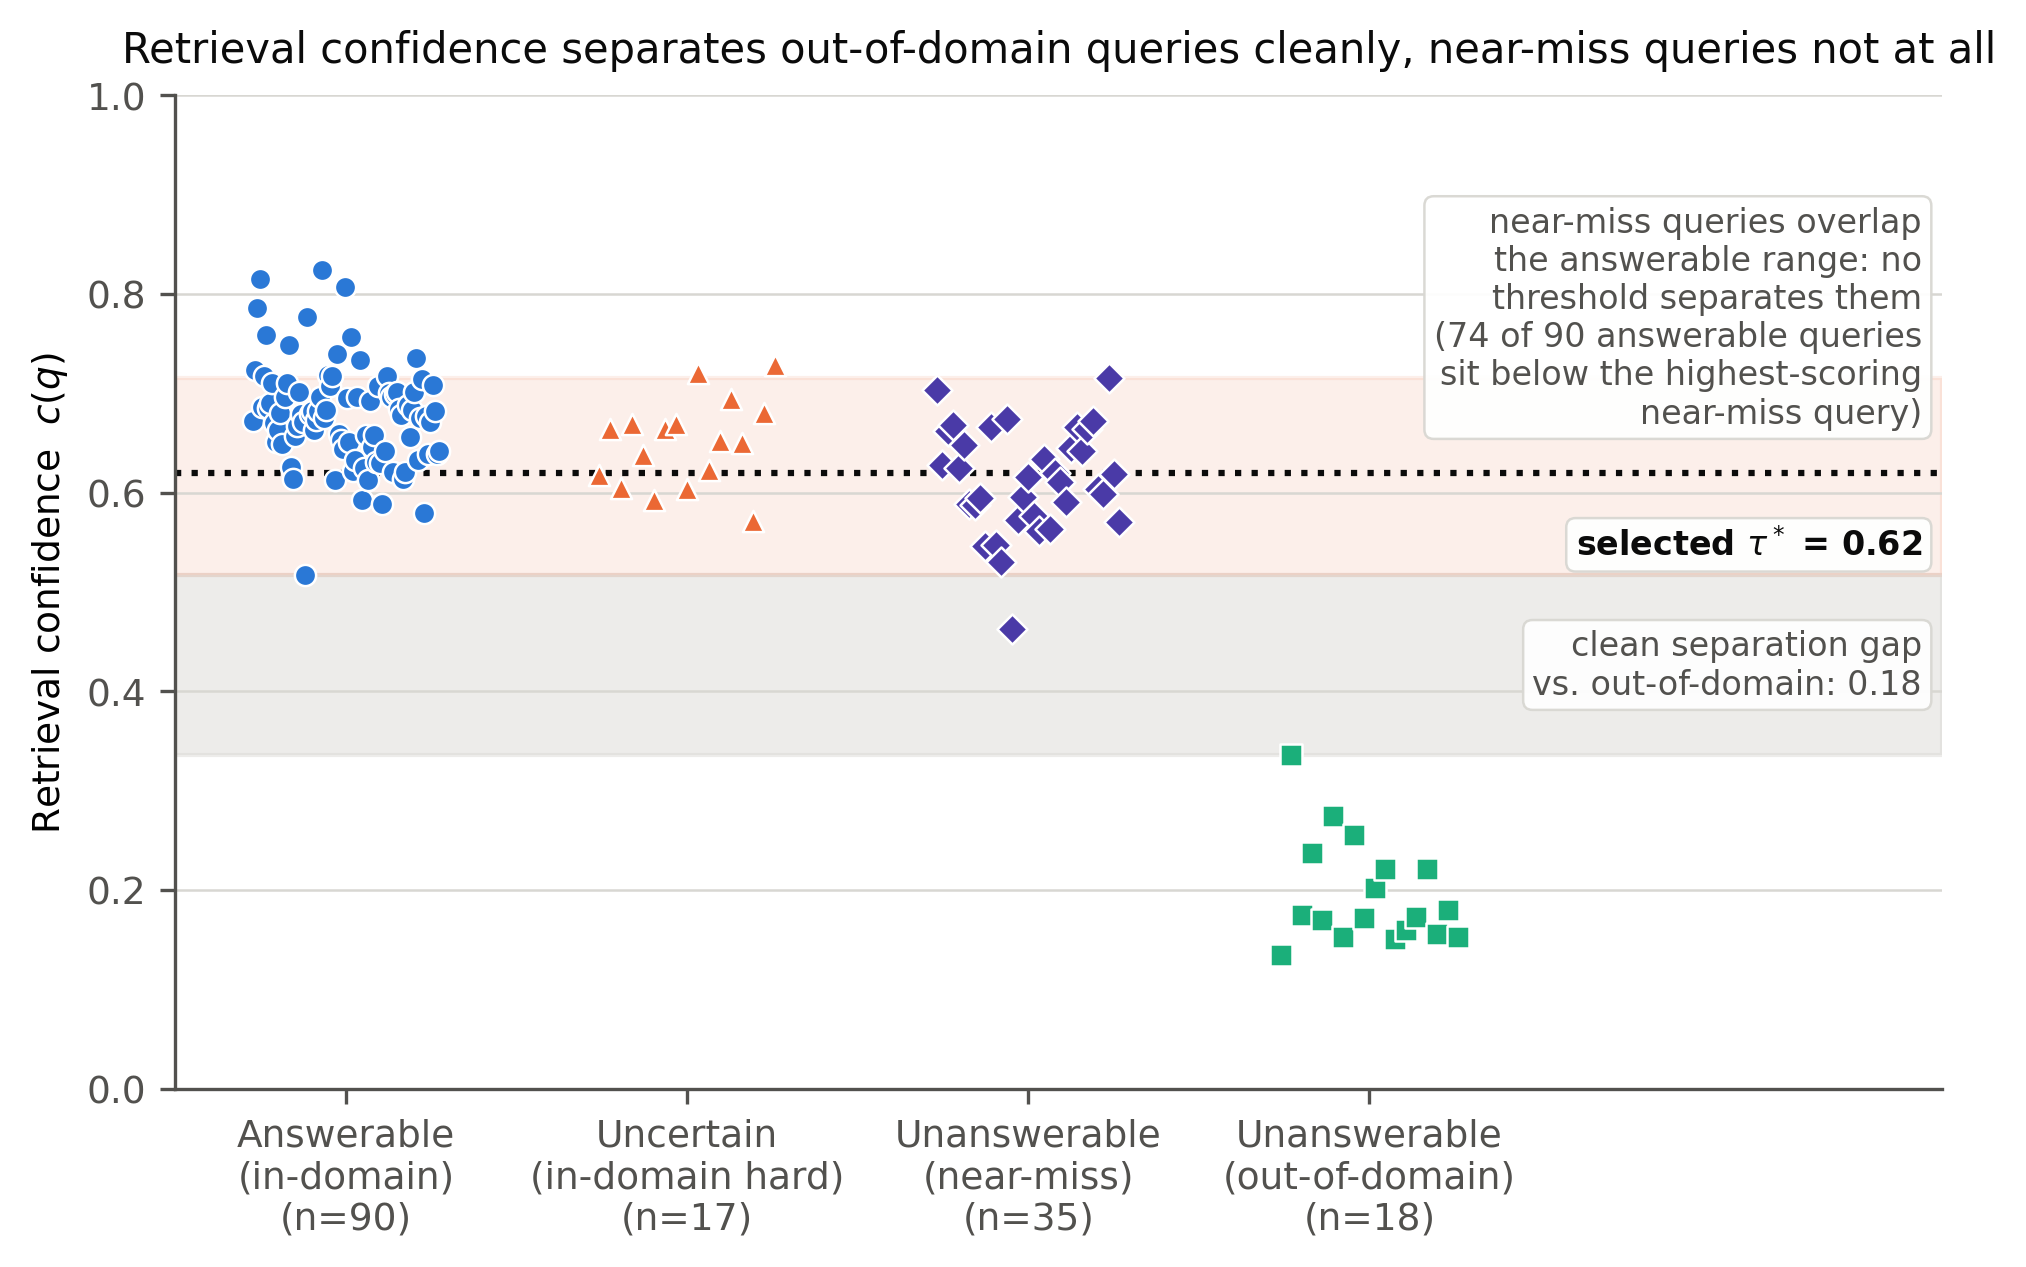
\includegraphics[width=0.78\linewidth]{figures/confidence_plot.png}
\caption{Retrieval confidence by ground-truth class, one point per query. Out-of-domain queries are separated from answerable ones by a clean margin of 0.18, so any threshold inside that band classifies all 108 correctly. Near-miss queries overlap the answerable range entirely --- 74 of the 90 answerable queries score no higher than the best near-miss --- so no scalar threshold separates those two classes at any operating point.}
\label{fig:confidence}
\end{figure*}

\subsection{Threshold Sweep}
\label{sec:sweep}

Table \ref{tab:sweep} and Fig. \ref{fig:threshold} give the sweep, and the shape is a genuine coverage--reliability tradeoff, which the overlap above implies it must be. Recall climbs monotonically: 0.00 at $\tau = 0.10$, 0.32 by 0.30, 0.72 at the selected threshold, saturating at 1.00 only by 0.75. Precision runs the other way, 1.00 from 0.15 (the first threshold at which the system abstains at all) through 0.50, falling to 0.38 by 0.80. The curves cross in the low 0.60s where MCC peaks at 0.65, which selects $\tau^\ast = 0.62$.

An earlier version of this study used only out-of-domain questions as its unanswerable class. Over that query set recall was pinned at 1.00 at every threshold, with only precision moving, and the natural conclusion was that the mechanism has no real tradeoff, only precision decay above a saturation point. That was an artifact of the evaluation set: add unanswerable questions that are hard rather than obvious and the tradeoff appears immediately. A sweep whose headline metric never moves has established nothing about that metric, and anyone reporting saturated abstention recall should check whether their unanswerable class is simply too easy.

Two further columns deserve a look. Effective relevance rises with $\tau$ from 3.30 to 5.00, but this is selection rather than improvement: as harder questions are abstained on, those remaining are on average easier. And the hallucination rate among substantive answers is roughly flat through the usable range, 0.12 to 0.08 between $\tau = 0.10$ and $\tau^\ast$, grounding the claim in Section \ref{sec:discussion} that the faithfulness gain comes from grounding rather than abstention.

\begin{table*}[t]
\centering
\caption{Threshold sweep (N = 160), showing representative thresholds from the sixteen swept. Abstention metrics are computed over the 143 queries with a definite answerability label. Faith.\ (ans.) is faithfulness over answered queries only; Hall.\ is the hallucination rate among substantive answers.}
\label{tab:sweep}
\begin{tabular}{@{}lcccccccccccc@{}}
\toprule
$\tau$ & Rel. & Eff.\ Rel. & Faith. & Faith.\ (ans.) & Abstain & Hall. & P & R & F1 & Spec. & Acc. & MCC \\
\midrule
0.10 & 3.30 & 3.30 & 3.58 & 3.58 & 0.00 & 0.12 & 0.00 & 0.00 & 0.00 & 1.00 & 0.63 & 0.00 \\
0.20 & 3.30 & 3.47 & 3.85 & 3.77 & 0.07 & 0.12 & 1.00 & 0.21 & 0.34 & 1.00 & 0.71 & 0.38 \\
0.30 & 3.30 & 3.57 & 4.00 & 3.88 & 0.11 & 0.12 & 1.00 & 0.32 & 0.49 & 1.00 & 0.75 & 0.48 \\
0.40 & 3.30 & 3.59 & 4.01 & 3.89 & 0.11 & 0.12 & 1.00 & 0.34 & 0.51 & 1.00 & 0.76 & 0.49 \\
0.50 & 3.30 & 3.61 & 4.04 & 3.91 & 0.12 & 0.12 & 1.00 & 0.36 & 0.53 & 1.00 & 0.76 & 0.51 \\
0.55 & 3.27 & 3.66 & 4.11 & 3.96 & 0.14 & 0.11 & 0.96 & 0.42 & 0.58 & 0.99 & 0.78 & 0.53 \\
0.60 & 3.22 & 3.93 & 4.33 & 4.11 & 0.24 & 0.11 & 0.89 & 0.62 & 0.73 & 0.96 & 0.83 & 0.64 \\
\textbf{0.62}$^\ast$ & \textbf{3.08} & \textbf{4.06} & \textbf{4.44} & \textbf{4.18} & \textbf{0.32} & \textbf{0.08} & \textbf{0.83} & \textbf{0.72} & \textbf{0.77} & \textbf{0.91} & \textbf{0.84} & \textbf{0.65} \\
0.65 & 2.76 & 4.36 & 4.62 & 4.27 & 0.47 & 0.07 & 0.65 & 0.83 & 0.73 & 0.73 & 0.77 & 0.54 \\
0.70 & 1.66 & 4.53 & 4.95 & 4.73 & 0.81 & 0.04 & 0.44 & 0.96 & 0.61 & 0.29 & 0.54 & 0.31 \\
0.75 & 1.18 & 5.00 & 5.00 & 5.00 & 0.96 & 0.00 & 0.39 & 1.00 & 0.56 & 0.08 & 0.42 & 0.17 \\
0.80 & 1.07 & 5.00 & 5.00 & 5.00 & 0.98 & 0.00 & 0.38 & 1.00 & 0.55 & 0.03 & 0.39 & 0.11 \\
\bottomrule
\end{tabular}
\end{table*}

\begin{figure}[tbp]
\centering
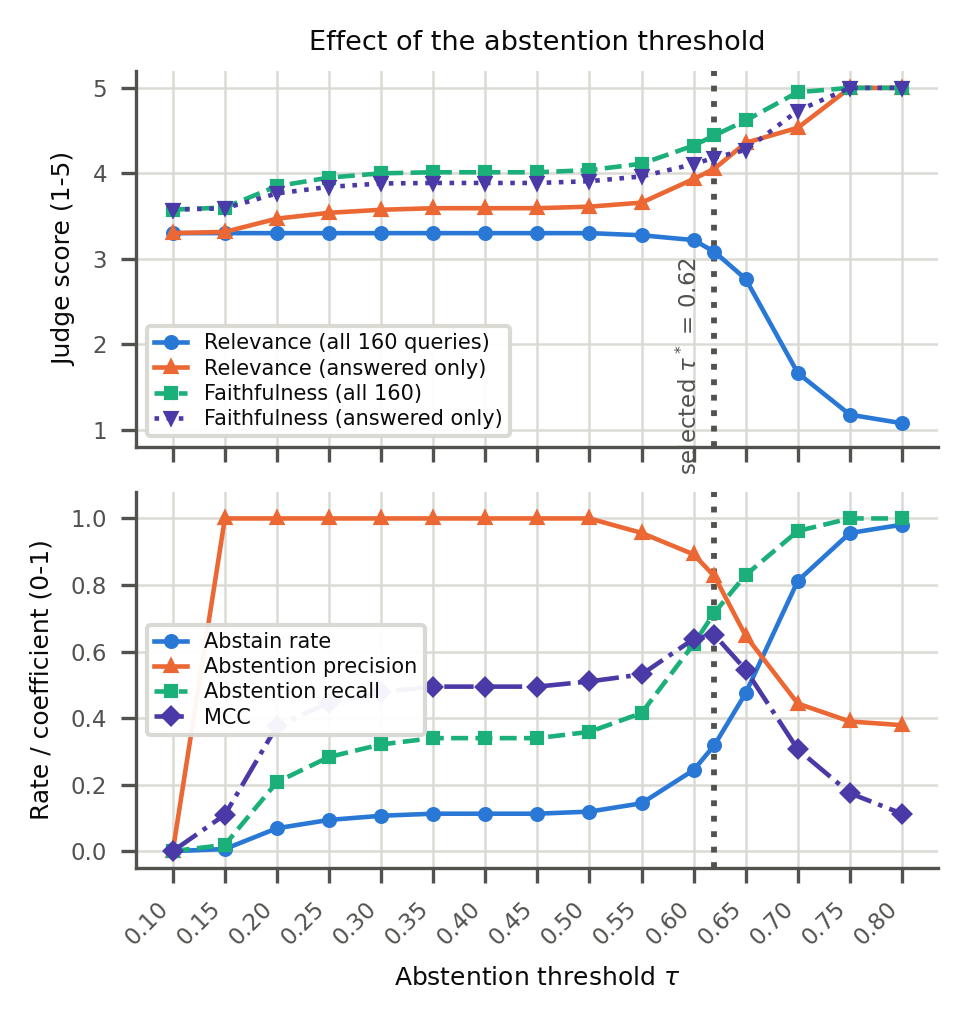
\includegraphics[width=\linewidth]{figures/threshold_plot.png}
\caption{Effect of the abstention threshold. Judge scores (1--5) above, rates and coefficients (0--1) below, sharing one $x$ axis. Precision and recall cross in the low 0.60s where MCC peaks; the dotted line marks $\tau^\ast = 0.62$, read from the selection script rather than annotated by hand.}
\label{fig:threshold}
\end{figure}

\subsection{The Decision at $\tau^\ast$, and a Second Refusal Channel}
\label{sec:categories}

At the selected threshold the confusion matrix over 143 labelled queries is TP = 38, FP = 8, TN = 82, FN = 15: precision 0.83, recall 0.72, F1 0.77, specificity 0.91, accuracy 0.84, MCC 0.65. Specificity of 0.91 says the mechanism is not trigger-happy, preserving nine of every ten answerable questions; recall of 0.72 is where the trouble is, and all 15 false negatives are near-miss questions, since every out-of-domain question is caught.

The category breakdown (Table \ref{tab:category}) tracks the separation analysis exactly: out-of-domain refused 100\% of the time, near-miss 57\%, and answerable categories between 0.07 and 0.13, the false-positive cost of operating at $\tau^\ast$.

The column worth dwelling on is generator refusals --- queries the gate passed on which the generator declined anyway. There are 25 among the 109 answered, unevenly spread: twelve near-miss and seven in-domain hard, so 19 of 25 fall in precisely the two categories the gate handles worst. The system therefore has two independent refusal channels failing in different places. The gate detects \emph{topic absence}; the generator detects \emph{claim absence}, noticing when passages are topically right but lack the specific fact. Neither alone suffices, and the second does quiet work a paper reporting only abstain rates would miss. It also explains why in-domain hard questions score 4.29 on faithfulness despite only 2.12 on relevance: they are largely not answered wrongly, they are not answered at all.

\begin{table}[htbp]
\centering
\caption{Results by category at $\tau^\ast = 0.62$. ``Gen.\ ref.'' counts queries the gate passed but the generator declined.}
\label{tab:category}
\begin{tabular}{@{}lcccccc@{}}
\toprule
Category & $n$ & Abst. & Gen.\ ref. & Rel. & Faith. & Mean $c(q)$ \\
\midrule
Factual & 40 & 0.07 & 1 & 4.62 & 4.67 & 0.691 \\
Reasoning & 20 & 0.10 & 2 & 4.20 & 4.50 & 0.670 \\
Comparative & 15 & 0.13 & 3 & 3.53 & 3.40 & 0.666 \\
Numeric & 15 & 0.07 & 0 & 4.73 & 4.73 & 0.669 \\
In-domain hard & 17 & 0.29 & 7 & 2.12 & 4.29 & 0.650 \\
Near-miss & 35 & 0.57 & 12 & 1.31 & 4.26 & 0.613 \\
Out-of-domain & 18 & 1.00 & 0 & 1.00 & 5.00 & 0.196 \\
\bottomrule
\end{tabular}
\end{table}

\subsection{Confident but Wrong}
\label{sec:failures}

Seven substantive answers passed the gate and were still judged unfaithful. Asked which franchise Red Chillies Entertainment owns, the system answered ``Lucknow Super Giants'' at confidence 0.663; the corpus says Kolkata Knight Riders. Asked how many teams played the inaugural season, it answered ``five'' at 0.675; the answer is eight. In both cases retrieval returned topically correct, high-scoring passages lacking the specific fact.

The sharpest case is a near-miss question. Asked \emph{``Which bowler has the best figures in an IPL match played on a Tuesday?''}, the system replied Axar Patel, 11 wickets for 70 against England on 13 February 2021, at confidence 0.642 --- a real record correctly transcribed from a retrieved passage, but from a Test match and nothing to do with Tuesdays. The text was topically plausible, the model assembled a fluent answer, and the gate had no basis to object. Catching this needs a signal about whether a specific claim is supported, not whether a topic is present.

\subsection{Confidence Variants and a Chance Baseline}

Table \ref{tab:variants} compares the three confidence definitions and adds a chance-level comparison. Neither alternative beats the mean: rank-weighting gives up recall (0.66 against 0.72) for a marginal specificity gain, ending at F1 0.74, and the maximum shifts the operating point rather than improving it, trading precision for recall at F1 0.75. The mean's advantage is small, but the negative result is worth reporting --- the obvious refinements do not rescue the mechanism, because the problem is not how the scores are combined. All three measure topical similarity, and near-miss queries are topically similar.

The chance baseline matters more. At $\tau^\ast$ the system abstains on 46 of 143 labelled queries, so we compared against abstaining on 46 chosen uniformly at random over 100 seeds. Random scores F1 0.35 and MCC 0.00 against the gate's 0.77 and 0.65. The mechanism is unambiguously doing real work, and saying so against an explicit chance level beats leaving the reader to guess what an F1 is worth on an imbalanced set.

\begin{table}[htbp]
\centering
\caption{Confidence definitions and chance-level abstention. The random row abstains on the same number of labelled queries as the gate does at $\tau^\ast$, averaged over 100 seeds.}
\label{tab:variants}
\begin{tabular}{@{}lcccccc@{}}
\toprule
$c(q)$ & $\tau^\ast$ & P & R & F1 & Spec. & MCC \\
\midrule
Mean (ours) & 0.62 & 0.83 & 0.72 & \textbf{0.77} & 0.91 & \textbf{0.65} \\
Rank-weighted & 0.62 & 0.83 & 0.66 & 0.74 & 0.92 & 0.62 \\
Maximum & 0.65 & 0.73 & 0.77 & 0.75 & 0.83 & 0.60 \\
\midrule
Random (chance) & -- & 0.37 & 0.32 & 0.35 & 0.68 & 0.00 \\
\bottomrule
\end{tabular}
\end{table}

\subsection{Validating the Judge}
\label{sec:judge-validation}

One author hand-scored 15 items against the same rubric the judge uses without looking at its scores first, drawn with a fixed seed, stratified across categories, with generator refusals excluded because faithfulness is undefined for an answer asserting nothing.

Agreement is substantial on both axes (Table \ref{tab:humanagreement}): Pearson $r$ of 0.83 for relevance and 0.85 for faithfulness, Spearman $\rho$ of 0.76 and 0.66, quadratic-weighted $\kappa$ of 0.80 and 0.83, mean absolute error 0.40, and 22 of 30 judgements matching exactly. We report $\kappa$ and $\rho$ alongside $r$ deliberately: ratings pile up at the ceiling, inflating exact-match rates and leaving $r$ determined by a handful of disagreements, whereas weighted $\kappa$ corrects for chance and penalises larger gaps. Of the eight disagreements, three are faithfulness cases where the human judged an answer better supported than the judge did, and three involve in-domain hard questions where crediting a partial answer is genuinely difficult; none exceeds two points. With $n = 15$ and one rater this establishes that the judge is not measuring something unrelated to human judgement, and no more.

\begin{table}[htbp]
\centering
\caption{Human vs.\ LLM-judge agreement ($n = 15$ items, 30 judgements)}
\label{tab:humanagreement}
\begin{tabular}{@{}lccccc@{}}
\toprule
Metric & MAE & Exact & Pearson $r$ & Spearman $\rho$ & $\kappa_w$ \\
\midrule
Relevance & 0.40 & 0.73 & 0.83 & 0.76 & 0.80 \\
Faithfulness & 0.40 & 0.73 & 0.85 & 0.66 & 0.83 \\
\bottomrule
\end{tabular}
\end{table}

\subsection{A Refusal Is Not a Hallucination}
\label{sec:refusals}

One finding emerged unasked for and changes how the headline metric must be computed. Across the run the generator produced 66 refusals, which the judge scored inconsistently: 42 received faithfulness 1, twenty-three received 5, and one received 3. The identical string \texttt{"I don't know."} drew all three scores on different queries, under one judge at temperature 0.

This is less the judge misbehaving than an ill-posed question: the rubric asks whether an assertion is supported by the context, and a refusal makes no assertion, so the judge answers differently each time. The consequence is concrete. Leaving refusals in the hallucination count pulls twelve below the cutoff, taking the RAG count from 7 to 19 --- an overstatement of roughly 170\% in the central reliability metric, driven by a rubric gap rather than anything the system did. We therefore exclude refusals from numerator and denominator alike, applying the same rule to RAG and baseline. This is also free, reproducible evidence about LLM-as-judge reliability: anyone using such a judge where refusals occur should check for this rather than assume it away.

\section{Discussion}
\label{sec:discussion}

\textbf{The difficulty of the unanswerable class determines what can be concluded.} With only off-topic questions, confidence separates perfectly and every metric saturates; add on-topic unanswerable questions and recall drops to 0.72 with no threshold available to fix it. Both results came from the same code, corpus and model, and only the evaluation set changed. Reported abstention performance is therefore a claim about the query set at least as much as about the method.

\textbf{Similarity-based confidence detects topic absence, not answer absence.} The score carries only the first, which sets a ceiling no amount of threshold tuning, rank weighting or swapping mean for max will lift, as Table \ref{tab:variants} shows. Getting past it needs a different signal: verification of the generated claim against the passages, or an uncertainty estimate from the generator. That the generator already refuses 19 of the hard cases unprompted suggests the second exists and is worth extracting deliberately.

\textbf{The faithfulness gain comes from grounding, not abstention.} It is tempting to credit the gate for the rise from 2.19 to 4.44, but the hallucination rate among substantive answers is roughly flat across the usable range of $\tau$, 0.12 to 0.08. Abstention removes queries that would have been answered ungroundedly; it does not improve the answers that remain. Grounding reduces hallucination and abstention reduces exposure, and a designer should know which they are buying.

The practical advice follows: measure the confidence distributions of your own answerable and unanswerable queries and check whether they overlap. If they separate, a wide range of thresholds works. If they overlap, no threshold is safe and the choice should be made against labelled answerability data rather than relevance and faithfulness curves, which vary smoothly and hide the structure underneath.

\section{Limitations}
\label{sec:limitations}

Everything here rests on one small, clean corpus of 62 encyclopedic pages, and we would expect the out-of-domain separation to be less crisp on messier text. With $n = 160$ and a single run we report point estimates without confidence intervals, so small differences between adjacent thresholds should not be over-read. The near-miss class is our own construction: verified against the corpus, but still our idea of what a hard unanswerable question looks like.

The confidence score is a raw cosine average rather than a calibrated probability, so the thresholds will not transfer numerically to another embedding model or corpus. The faithfulness rubric is partly circular for abstentions, assigned 5 by definition --- hence effective faithfulness throughout --- and undefined for refusals, which we handle by exclusion: a decision, not a measurement. The human validation is 15 items and one rater. Hit@$k$ and Precision@$k$ rely on substring matching against hand-written keywords, which we did not tune. Finally, retrieval is a single dense pass: a cross-encoder reranker \cite{nogueira2019passage} or BM25 hybrid \cite{robertson2009bm25} would likely lift Precision@3 above 0.73, and since that residual is where the confident-but-wrong answers originate, might reduce them.

\section{Conclusion and Future Work}

We studied confidence-gated abstention for RAG on a 160-question set built to contain unanswerable questions of two difficulties. Against a no-context baseline, faithfulness rises from 2.19 to 4.44 and the hallucination rate falls from 0.62 to 0.08; scored as classification against ground truth, the abstention decision reaches F1 0.77 and MCC 0.65, well clear of a chance-matched 0.35 and 0.00.

The more useful finding concerns the method's boundary. Retrieval confidence separates off-topic questions from answerable ones with a clean margin and catches all of them, but does not separate near-miss questions at all: 74 of 90 answerable questions score no higher than the best near-miss, and no threshold fixes this. A threshold on retrieval similarity can tell you a topic is missing from your corpus; it cannot tell you an answer is missing from a topic that is present.

The most direct next step is to extract the generator's own refusal behaviour as a deliberate second signal, with claim-level verification against the retrieved passages as the thorough version. Beyond that: repeating the study where the domain boundary is blurry, adding reranking, calibrating the score so thresholds transfer, and a larger multiply-annotated judge validation. Code, the labelled query set, the corpus and the scripts regenerating every table and figure are in the project repository.

\begin{thebibliography}{00}

\bibitem{lewis2020rag} P. Lewis et al., ``Retrieval-Augmented Generation for Knowledge-Intensive NLP Tasks,'' in \emph{Advances in Neural Information Processing Systems (NeurIPS)}, 2020.

\bibitem{rajpurkar2018know} P. Rajpurkar, R. Jia, and P. Liang, ``Know What You Don't Know: Unanswerable Questions for SQuAD,'' in \emph{Proc. of ACL}, 2018.

\bibitem{ji2023survey} Z. Ji et al., ``Survey of Hallucination in Natural Language Generation,'' \emph{ACM Computing Surveys}, vol. 55, no. 12, 2023.

\bibitem{reimers2019sentencebert} N. Reimers and I. Gurevych, ``Sentence-BERT: Sentence Embeddings using Siamese BERT-Networks,'' in \emph{Proc. of EMNLP}, 2019.

\bibitem{johnson2019faiss} J. Johnson, M. Douze, and H. J\'egou, ``Billion-scale similarity search with GPUs,'' \emph{IEEE Transactions on Big Data}, 2019.

\bibitem{zheng2023judging} L. Zheng et al., ``Judging LLM-as-a-Judge with MT-Bench and Chatbot Arena,'' in \emph{Advances in Neural Information Processing Systems (NeurIPS)}, 2023.

\bibitem{robertson2009bm25} S. Robertson and H. Zaragoza, ``The Probabilistic Relevance Framework: BM25 and Beyond,'' \emph{Foundations and Trends in Information Retrieval}, vol. 3, no. 4, pp. 333--389, 2009.

\bibitem{nogueira2019passage} R. Nogueira and K. Cho, ``Passage Re-ranking with BERT,'' arXiv:1901.04085, 2019.

\bibitem{asai2024selfrag} A. Asai, Z. Wu, Y. Wang, A. Sil, and H. Hajishirzi, ``Self-RAG: Learning to Retrieve, Generate, and Critique through Self-Reflection,'' in \emph{Proc. ICLR}, 2024.

\bibitem{es2024ragas} S. Es, J. James, L. Espinosa-Anke, and S. Schockaert, ``RAGAs: Automated Evaluation of Retrieval Augmented Generation,'' in \emph{Proc. EACL: System Demonstrations}, 2024, pp. 150--158.

\bibitem{guo2017calibration} C. Guo, G. Pleiss, Y. Sun, and K. Q. Weinberger, ``On Calibration of Modern Neural Networks,'' in \emph{Proc. ICML}, 2017.

\bibitem{kadavath2022know} S. Kadavath et al., ``Language Models (Mostly) Know What They Know,'' arXiv:2207.05221, 2022.

\end{thebibliography}

\end{document}
